\documentclass{assignment}
\ProjectInfos{光电子技术}{PHYS6651P}{2021-2022学年第一学期}{第八章作业}{}{陈稼霖}[https://github.com/Chen-Jialin]{SA21038052}

\begin{document}
\begin{prob}
    图示一种相位型光纤温度传感器原理图,从两光纤末端输出的两光波在空间叠加形成明暗相间的杨氏条纹. 当信号臂的温度发生变化时,输出两端光波的相位差发生改变($\Delta\varphi$)表示,于是屏上条纹发生移动,观测条纹移动数便可求得温度的变化量,并有公式如下:$\varphi/(\Delta T\cdot L)=2\pi/\lambda(\Delta n/\Delta T+n\Delta L/(L\Delta T))$. 如果光源 $\lambda=6328$ \AA,光纤的折射率 $n=1.456$,$\mathrm{d}n/\mathrm{d}T=10\times 10^{-6}/^{\circ}$C,$\alpha=\Delta L/(L\cdot\Delta T)=5\times 10^{-7}/^{\circ}$C,光纤长度 $L=1$ 米,求对应一个条纹间隔变化时的温度的变化.
    \begin{figure}[h]
        \centering
        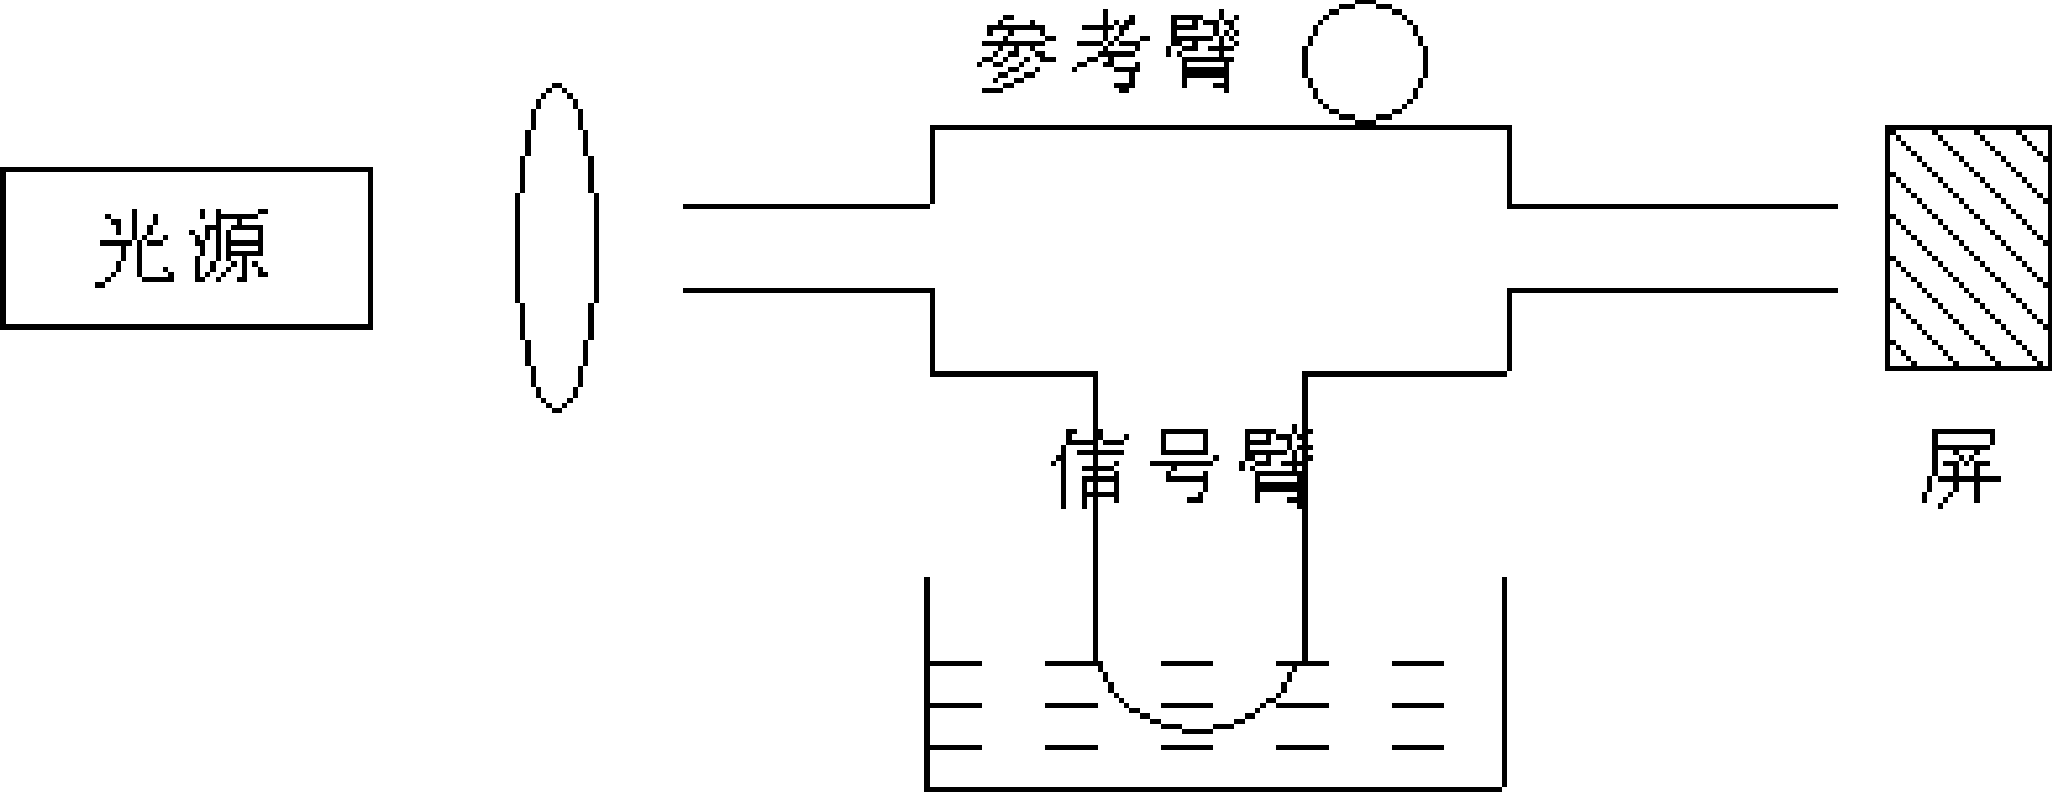
\includegraphics[width=.5\columnwidth]{4-1.png}
    \end{figure}
\end{prob}
\begin{sol}
    一个条纹间隔变化对应 $\Delta\varphi=\pi$ 的相移, 即
    \begin{gather}
        \frac{\Delta\varphi}{L\cdot\Delta T}=\frac{2\pi}{\lambda}\left(\frac{\Delta n}{\Delta T}+\frac{n}{L}\frac{\Delta L}{\Delta T}\right),\\
        \Longrightarrow\frac{\pi}{1\text{ m}\cdot\Delta T}=\frac{2\pi}{6.328\times 10^{-7}\text{ m}}\left(10\times 10^{-6}/{}^\circ\text{C}+1.456\times 5\times 10^{-7}/{}^{\circ}\text{C}\right),\\
        \Longrightarrow\Delta T=0.029^{\circ}\text{C}.
    \end{gather}
    故一个条纹间隔变化时温度变化 $0.029^{\circ}$C.
\end{sol}

\begin{prob}
    全光纤马赫-泽德(M-Z)滤波器通常是由两个 $3$ dB 耦合器连接而成,如下图所示,定向耦合器的传输矩阵为 $\begin{bmatrix}
        \sqrt{1-C}&-j\sqrt{C}\\
        -j\sqrt{C}&\sqrt{1-C}
    \end{bmatrix}$,光纤段的传输矩阵为 $\begin{bmatrix}
        \exp(-jk_0nl_1)&0\\
        0&\exp(-jk_0nl_2)
    \end{bmatrix}$,其中 $C$ 为耦合效率($3$ dB 相当于 $C=0.5$),$l_1$ 和 $l_2$ 为中间光纤臂长,设光场从 1 端输入,求从 3、4 端出射的光场振幅透射系数 $T_{13}$ 和 $T_{14}$ 及相邻透射峰之间的波长差.
    \begin{figure}[h]
        \centering
        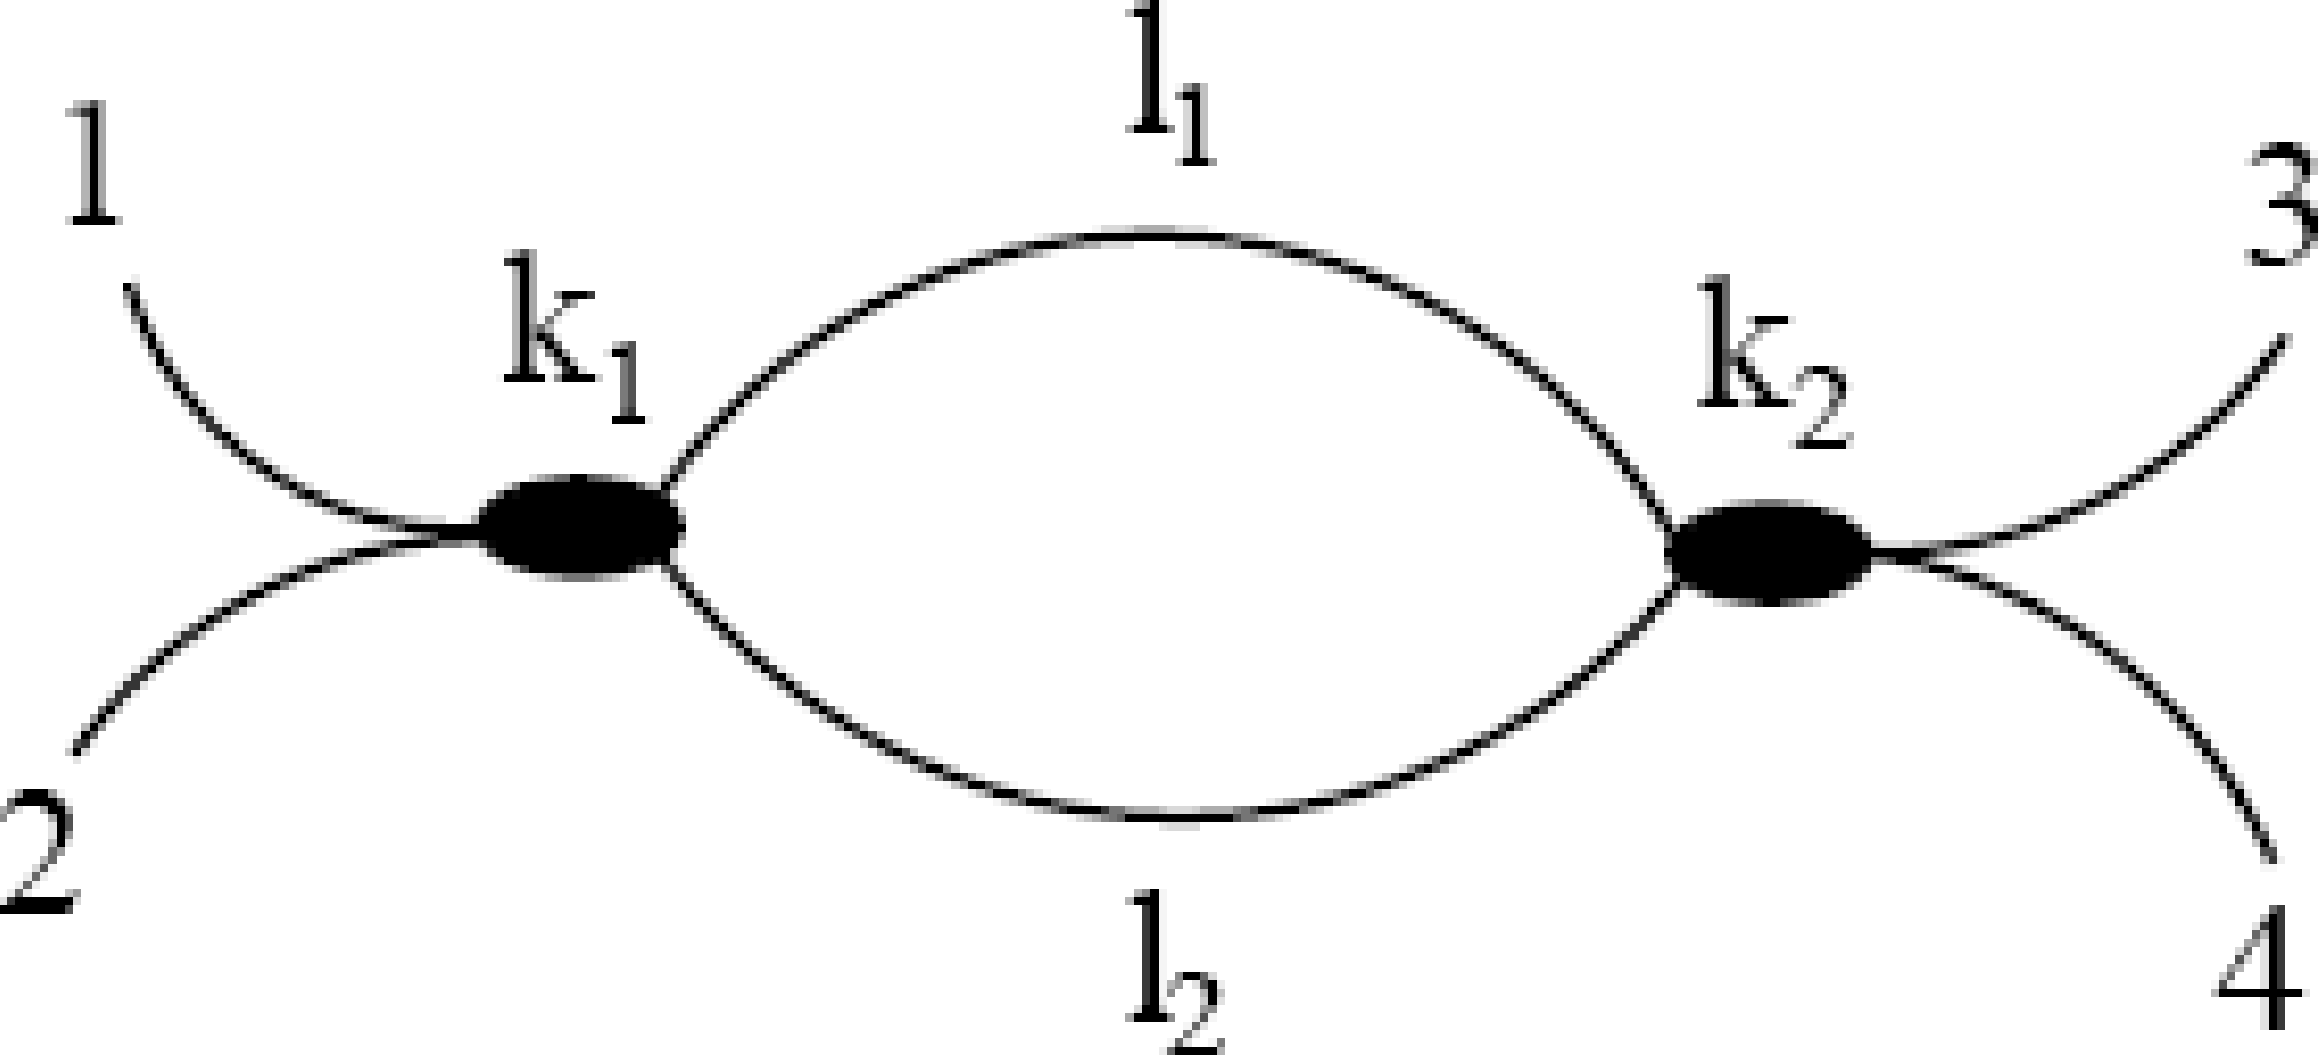
\includegraphics[width=.5\columnwidth]{4-3.png}
    \end{figure}
\end{prob}
\begin{sol}
    当光场从 1 端以幅度 $E_1$ 输入, 从 3、4 端出射的幅度 $E_3,E_4$ 分别为
    \begin{align}
        \notag\begin{bmatrix}
            E_3\\
            E_4
        \end{bmatrix}=&\frac{1}{\sqrt{2}}\begin{bmatrix}
            1&-j\\
            -j&1
        \end{bmatrix}\begin{bmatrix}
            \exp(-jk_0nl_1)&0\\
            0&\exp(-jk_0nl_2)
        \end{bmatrix}\frac{1}{\sqrt{2}}\begin{bmatrix}
            1&-j\\
            -j&1
        \end{bmatrix}\begin{bmatrix}
            E_1\\
            0
        \end{bmatrix}\\
        % \notag=&\frac{1}{2}\begin{bmatrix}
        %     \exp(-jk_0nl_1)-\exp(-jk_0nl_2)&-j[\exp(-jk_0nl_1)+\exp(-jk_0nl_2)]\\
        %     -j[\exp(-jk_0nl_1)+\exp(-jk_0nl_2)]&-\exp(-jk_0nl_1)+\exp(-jk_0nl_2)
        % \end{bmatrix}\begin{bmatrix}
        %     E_1\\
        %     0
        % \end{bmatrix}\\
        \notag=&\frac{E_1}{2}\begin{bmatrix}
            \exp(-jk_0nl_1)-\exp(-jk_0nl_2)\\
            -j[\exp(-jk_0nl_1)+\exp(-jk_0nl_2)]
        \end{bmatrix}\\
        =&-jE_1\exp\left(-jkn_0\frac{l_1+l_2}{2}\right)\begin{bmatrix}
            \sin\left(k_0n\frac{\Delta L}{2}\right)\\
            \cos\left(k_0n\frac{\Delta L}{2}\right)
        \end{bmatrix},
    \end{align}
    其中 $\Delta L=l_1-l_2$.
    从 3、4 端出射的光场透射系数分别为
    \begin{align}
        T_{13}=&\abs{\frac{E_3}{E_1}}^2=\sin^2\left(k_0n\frac{\Delta L}{2}\right)=\frac{1-\cos(2\pi n\Delta L/\lambda)}{2},\\
        T_{41}=&\abs{\frac{E_4}{E_1}}^2=\cos^2\left(k_0n\frac{\Delta L}{2}\right)=\frac{1+\cos(2\pi n\Delta L/\lambda)}{2}.
    \end{align}

    设相邻透射峰对应的波长分别为 $\lambda_1$, $\lambda_2$, 则
    \begin{align}
        \frac{2\pi n\Delta L}{\lambda_1}=&2n\pi,\\
        \frac{2\pi n\Delta L}{\lambda_2}=&(2n+1)\pi,
    \end{align}
    以上两式相减得
    \begin{gather}
        2\pi n\Delta L\left(\frac{1}{\lambda_2}-\frac{1}{\lambda_1}\right)=\pi,\\
        \Longrightarrow\lambda_1-\lambda_2=\frac{\lambda_1\lambda_2}{2n\Delta L}.
    \end{gather}
\end{sol}
\end{document}